%%%%%%%%%%%%%%%%%%%%
%% KAPITEL Server %%
%%%%%%%%%%%%%%%%%%%%
%% STEFFEN
%%%%%%%%%%%%%%%%%%%%%
\section{Einleitung}
% kurze Grundlage, dass man Server braucht (sowohl Applikationsserver -> für ERP,...; als auch Storageserver, wo Daten abgelegt werden (!=App. Server => Redudanz), als auch welche Betriebssysteme von SAP grundsätzlich unterstützt werden
\section{SAP GUI}
\label{sec:sapgui}

\section{SAP NetWeaver Plattform}
\label{sec:netweaver}

%%%%%%%%%%%%%%%%%%%%%%%
%% KAPITEL Datenbank %%
%%%%%%%%%%%%%%%%%%%%%%%
%% STEFFEN
%%%%%%%%%%%%%%%%%%%%%%%
\section{Datenbanken}

\subsection{SAP HANA}
\label{sec:db-hana}

\subsubsection{Einführung}
\label{sec:db-hana-intro}
% historische, hana studio, rowstore (anderer Aufbau als bei herkömml. dbs)
\gls{sap} \gls{hana} kombiniert die Funktionen einer \gls{db}, der Datenverarbeitung und die Funktionen einer Anwendungsplattform auf Ebene des Hardware Arbeitsspeichers. \gls{hana} bietet \gls{ua} Bibliotheken für Vorhersage, Planung, Textanalyse oder Geschäftsanalysen an.\\

\begin{figure}[H]
	\begin{center}
	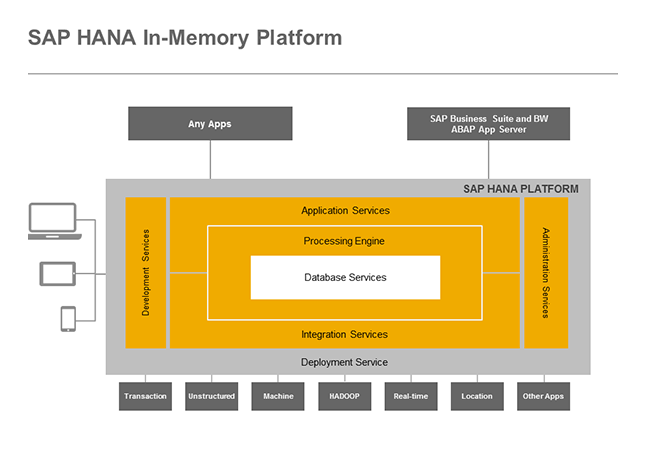
\includegraphics[width=1\linewidth]{grafiken/hana-features-overview.png}
	\vspace{-20pt}
	\caption{Aufbau der \gls{sap} \gls{hana} Plattform \cite{SAPHanaAbout}}
	\vspace{-10pt}
	\label{abb:SAPHanaAbout}
	\end{center}
\end{figure}

\gls{hana} verwendet in seiner \gls{db} einen sogenannten spaltenbasierten Datenspeicher, welcher im Arbeitsspeicher abgespeichert wird. Dieser Datenspeicher ist durch verschiedene Sicherheitsfeatures vor Datenverlust bei Stromausfall oder ähnlichem gesichert.
Dadurch, dass Anwendungen direkt auf der \gls{hana} Instanz ausgeführt werden können, vereinfacht es die Entwicklung von Applikationen im Umfeld von großen Datenquellen und Datenstrukturen. In Abbildung \ref{abb:SAPHanaAbout} ist die Struktur von \gls{hana} abgebildet.

\subsubsection{Hands On}
\label{sec:db-hana-ho}
% welche wichtigen Befehle gibt es
Für dieses Kapitel wurde eine \gls{hana} Instanz von Grund auf konfiguriert und für den Einsatz vorbereitet. 
Als Grundlage für unser Testsystem dient ein mit VMWare virtualisierter Server mit folgenden Spezifikationen
\begin{itemize}
	\item \gls{cpu} \ldots Intel(R) Xeon(R) CPU E7- 4870  @ 2.40GHz mit 10vCores
	\item \gls{ram} \ldots 127 Gigabyte
	\item \gls{hdd} \ldots 180 Gigabyte
	\item \gls{os} \ldots Suse Enterprise Linux 11.2	
\end{itemize}

Aufgrund von Komplexitäts- und Zeitgründen gehe ich an dieser Stelle nicht weiter auf die Installation der \gls{hana} Instanz ein, lediglich ist zu erwähnen, dass man gewisse Instanz Attribute zum späteren Login benötigt. Dies sind \gls{ua} \emph{Instance}, \emph{Sid} und natürlich Logindaten für den \emph{System} Benutzer.\\
Zum benutzen der \gls{hana} Instanz benötigt man das Programm "`\gls{sap} \gls{hana} Studio"'. Dieses steht unter folgendem Link\footnote{\url{http://scn.sap.com/community/developer-center/hana}} zum Download zur Verfügung.

Nachdem das System im \gls{hana} Studio (mithilfe der Instanz Attribute) hinzugefügt wurde, können alle Funktionen von \gls{hana} verwenden werden.

Zunächst befüllen wir eine Datenbank mit mehreren Tabellen, die mit Hilfe eines \gls{sql} Scripts mit Zufallsdaten gefüllt werden (siehe \ref{anhang:hanasql}). In unserem Beispiel werden 10 Millionen Datensätze eingefügt. Aufgrund der Komplexität des Scripts dauerte das Einfügen auf der Instanz mehr als 40 Stunden. Dies kann je nach Hardware variieren.\\

\lstset{language=SQL, caption={Beispieldaten selektieren}, label={hana:select}}								
\begin{lstlisting}
SELECT * FROM "SYSTEM"."TABELLENNAME"
\end{lstlisting}

Um alle 10 Millionen Datensätze zu selektieren  (siehe \ref{hana:select}), benötigt die \gls{hana} \gls{db} lediglich weniger als 285 Millisekunden. Dies zeigt, dass auch weitaus mehr Datensätze selektiert und damit Anwendungen exponentiell verschnellert werden können. Wie sich \gls{hana} im Vergleich mit anderen herkömmlichen Datenbanken verhält, wird in Kapitel \ref{sec:db-hana-vgl} behandelt.

\begin{verbatim}
Statement 'SELECT * FROM "SYSTEM"."SALES_F"' 
successfully executed in 284 ms 214 µs  (server processing time: 275 ms 793 µs)
\end{verbatim}


\subsubsection{Vergleich}
\label{sec:db-hana-vgl}
% zeitvergleich oracle / hana db select

\subsection{Sonstige}
\label{sec:db-sonstige}
% welche datenbanken kann man sonst benutzen
% oracle,...